\section{Results and Discussion}
\label{sec:results}

In this section we present the main findings of our research. We first present the results of each study (Section~\ref{sec:survey-resuts}, Sections~\ref{sec:msr-results}, and Section~\ref{sec:interview-results}). After that, in Section~\ref{sec:discussion} we consolidate our findings and present some implications of our study. 

\subsection{Results of the first study: a survey}
\label{sec:survey-resuts} 

Our first study aims to investigate the impact of atoms of confusion while developers try to understand JavaScript code. We estimate this impact considering two perspectives: \emph{misunderstanding rate} (number of wrong answers) and \emph{cognitive effort} (time necessary to provide an answer). As discussed in section~\ref{sec:survey-settings}, 140 participants answered the survey in full. Figure~\ref{fig:degree} and Figure~\ref{fig:xp} show the distributions of the subjects, according to their education level and years of programming experience, respectively.

\begin{figure}[htb]
      \centering
      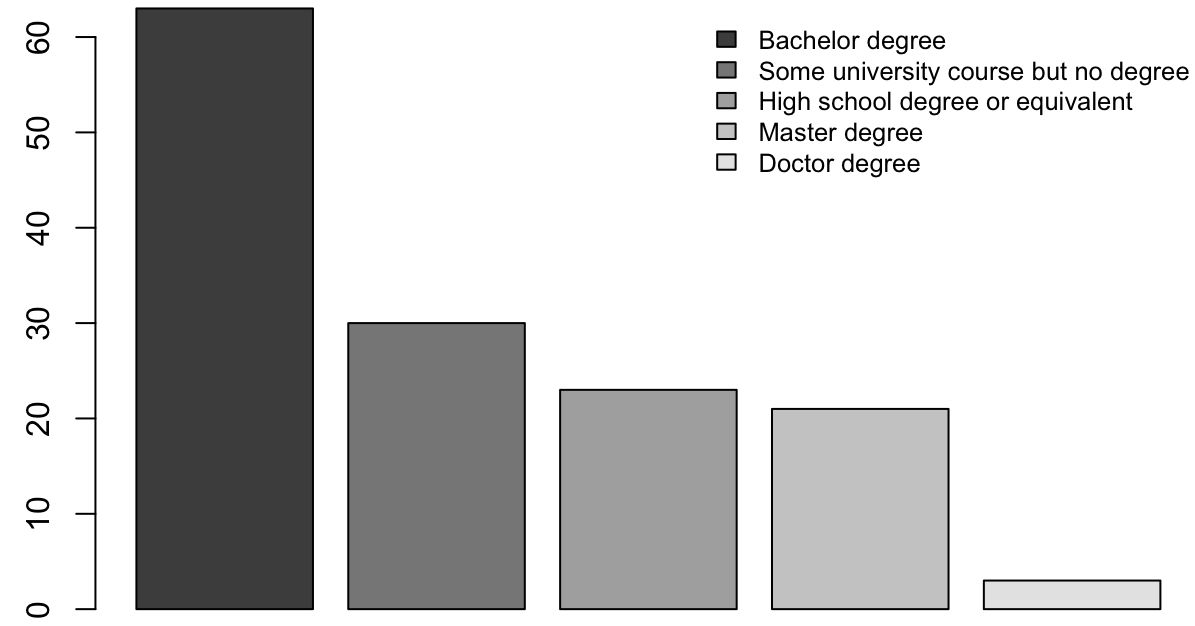
\includegraphics[scale=.25]{images/degree.png}
      \caption{Participants' Education Level}\label{fig:degree}
  \end{figure}
  
  \begin{figure}[htb]
      \centering
      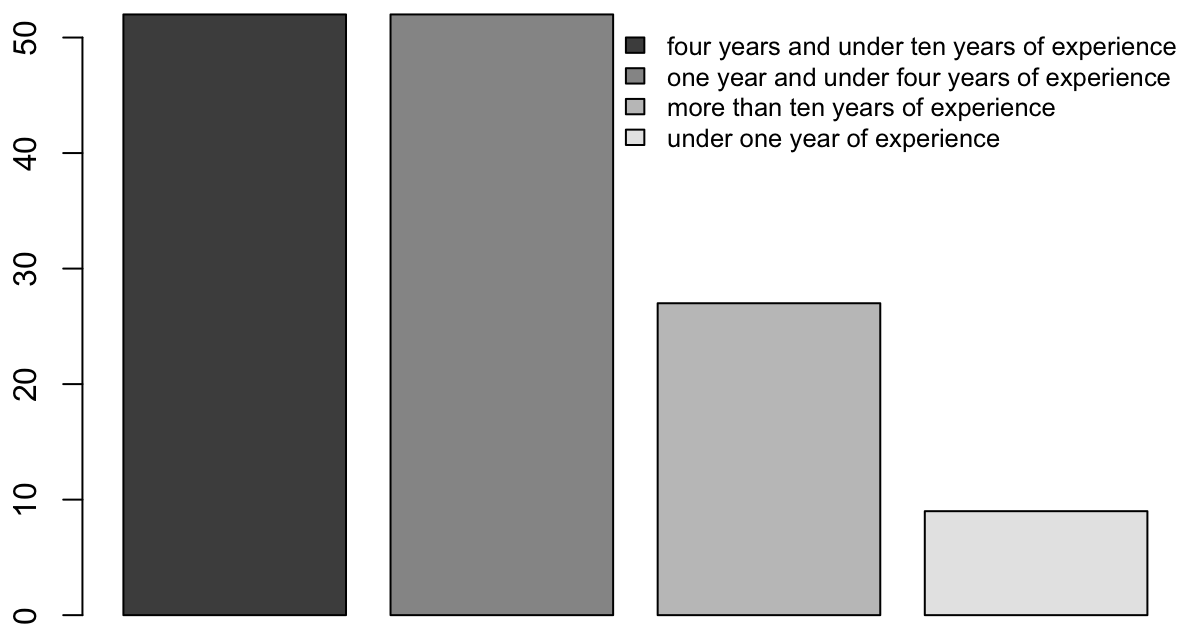
\includegraphics[scale=.25]{images/experience.png}
      \caption{Participants' Experience} \label{fig:xp}
  \end{figure}

It is possible to realize in Figure \ref{fig:xp} that more than a half of the participants hold either a BS degree or had taken some university course, meaning the participants have had some level of formal education on programming. No subject reported to have never attended university. Out audience comprises experience developers, and 93\% of the respondents have more than one year of experience with programming (see Figure~\ref{fig:xp}). Actually, 56\% of the participants have either between four and ten years of experience (37\%) or more than ten years of experience (19\%). Other 37\% of the respondents have between one and four years of experience. In this way, we can characterize the effect of atoms of confusion in JavaScript code taking into account the perceptions of both novice and experience developers. 

Each participant in this study evaluated {\color{red}10} code snippets, from which 5 were in their confusing versions, whilst the other 5 contained simplified versions of the code snippets (i.e., without the confusing constructs and idioms). The participants should provide the expected outcomes of the code snippets. We collected information about \emph{correctness} (whether the participant correctly predicted the program's output) and \emph{cognitive workload} (the time taken to answer the question). Our final dataset consists of 70 complete Latin Squares, which means that our assessment consider a total of 140 answers to each pair of code snippets.


Regarding \emph{correctness}, Table~\ref{results_correctness} and Figure~\ref{fig:boxplotcorrectness} summarize the results of the survey. Accordingly, the version of seven code snippets without atoms of confusion present at least a 15\% improvement in answer correctness. In particular, \emph{Comma Operator} atom presents the highest impact on misunderstanding. 
Curiously, frequently used constructs and idioms, such as \emph{Post Increment} and \emph{Omitted Curly Braces} (see Section~\ref{sec:msr-results}), also introduce high degrees of confusion. As the boxplot in Figure \ref{fig:boxplotcorrectness} shows, there is a considerable decrease in the average number of incorrect answers when the atoms were not present. Also, the sample of answers where there was no atoms had almost no dispersion, which is a sign that the non-confusing code is easier to evaluate correctly.

% \begin{table}[htbp]
% \caption{Difference in answer correctness between confusing and non-confusing pairs}
% \begin{center}
% \begin{small}
% \begin{tabularx}
% {{\linewidth}}{l p{1.5cm} p{1.1cm} p{1.1cm} p{1.2cm} }
% \textbf{Atom} & \textbf{\%Correct} & \textbf{\%Correct} \\
% &  \multicolumn{1}{l}{With AOC} \multicolumn{2}{l}{Without AOC}  & \Delta (\%)    \\
%  \hline
% Comma Operator & 40 & 93 & +132\%                 \\     
% Automatic Semicolon  Insertion & 46 & 97 & +110\% \\
% Post Increment & 69 & 91 & +31\%         \\
% Omitted Curly Braces & 67 & 83 & +23\%   \\ 
% Assignment as Value & 80 & 97 & +21\%    \\
% Implicit Predicate & 83 & 97 & +16\%     \\
% Logic as Control Flow & 59 & 68 & +15\%  \\
% Ternary Operator & 86 & 94 & +9\%        \\
% Pre-Increment & 71 & 76 & +7\%           \\
% Arithmetic as Logic & 91 & 90 & -1\%    \\
% \end{tabularx}
% \end{small}
% \end{center}
% \label{results_correctness}
% \end{table}

\begin{table}[htbp]
\caption{Average number of correct answers.}
\label{tab:difference-correctness}
\begin{tabular}{lccc} \toprule
 & \multicolumn{2}{c}{Average Number of Correct Answers} & \\ [0.1cm]
 Atom & Code with Atoms & Code without Atoms & $\Delta$(\%) \\ \midrule 
 Comma Operator          & 40 & 93  & +132 \\
 Post Increment          & 69 & 91  & + 31  \\
 Omitted Curly Braces    & 67 & 83  & +23 \\
 Assignment as Value     & 80 & 97  & +21 \\
 Implicit Predicate      & 83 & 97  & +16 \\
 Logic as Control Flow   & 59 & 68  & +15 \\
 Ternary Operator        & 86 & 94  & +9  \\
 Pre-Increment           & 71 & 76  & +7  \\
 Arithmetic as Logic     & 91 & 90  & +1  \\ \bottomrule
\end{tabular}
\end{table}


\begin{figure}[htb!]
\noindent
 \centering
 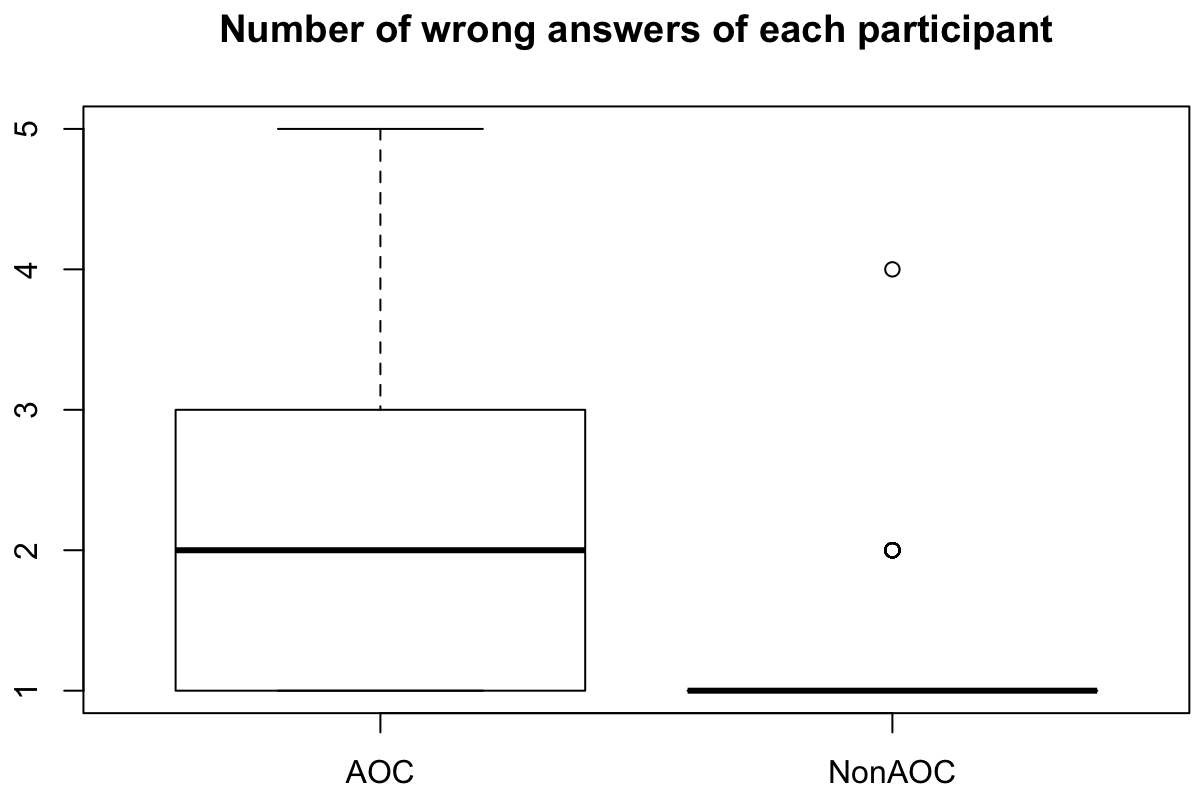
\includegraphics[scale=.20]{images/wrong.png}
 \caption{Number of wrong answers of each subject}
 \label{fig:boxplotcorrectness}
 \end{figure}

\rb{verificar a consistencia nas questoes de pesquisa mais especificas}
Regarding the first question we 
address in the survey (\emph{Do code snippets that contain atoms of confusion produce a higher error rate than snippets where the atom is removed?}), we found evidence that the atoms of confusion lead programmers to misunderstand JavaScript code. We also realized that just one atom whose correction has a non-significant improvement in the percentage of correct answers---we found an improvement of at least 15\% in the correct answers when removing the confusing code for seven atoms (out of ten atoms we consider in the survey). 

\rb{acho que valeria a pena colocar o teste de hipotese aqui}
\adriano{como fazemos/descrevemos o teste?}

Table \ref{tab:difference-time-taken} displays the results of the measurements of the average time taken to answer with and without atoms of confusion. Once again, the \emph{Comma Operator} was the construct whose removal had the greatest impact. The more expressive results in this measurement are the ones regarding \emph{Logic as Control Flow}, \emph{Implicit Predicate} and \emph{Omitted Curly Braces}, {\color{blue}as they are frequent in JavaScript libraries}. 

\rb{n\~{a}o sei se devemos antecipar o resultado do estudo de minera\c c\~{a}o 
nessa se\c c\~{a}o. talvez nao comprometa tanto.}

Figure \ref{fig:timetoanswer} shows a box plot of the difference in time taken the predict the output of average time to assess the code snippets. Although the dispersion is smaller for non-confusing code blocks, the median time did not vary much.


\begin{table}[htbp]
\caption{Average number of correct answers.}
\label{tab:difference-time-taken}
\begin{tabular}{lccc} \toprule
 & \multicolumn{2}{c}{Average Time in Seconds to Answer} & \\ [0.1cm]
 Atom & Code with Atoms & Code without Atoms & $\Delta$(\%) \\ \midrule 
Comma Operator        & 60 & 21  & -65  \\
Logic as Control Flow & 85 & 49  & -42  \\
Implicit Predicate    & 33 & 24  & -27  \\
Omitted Curly Braces  & 43 & 31  & -27  \\
Assignment as Value   & 53 & 49  & -7   \\
Ternary Operator      & 42 & 42  & 0    \\
Post Increment        & 27 & 27  & 0    \\
Arithmetic as Logic   & 29 & 36  & +24  \\
Pre-Increment         & 34 & 49  & +44  \\
         \bottomrule
    \end{tabular}
\end{table}

\begin{figure}[htb!]
      \noindent
      \centering
      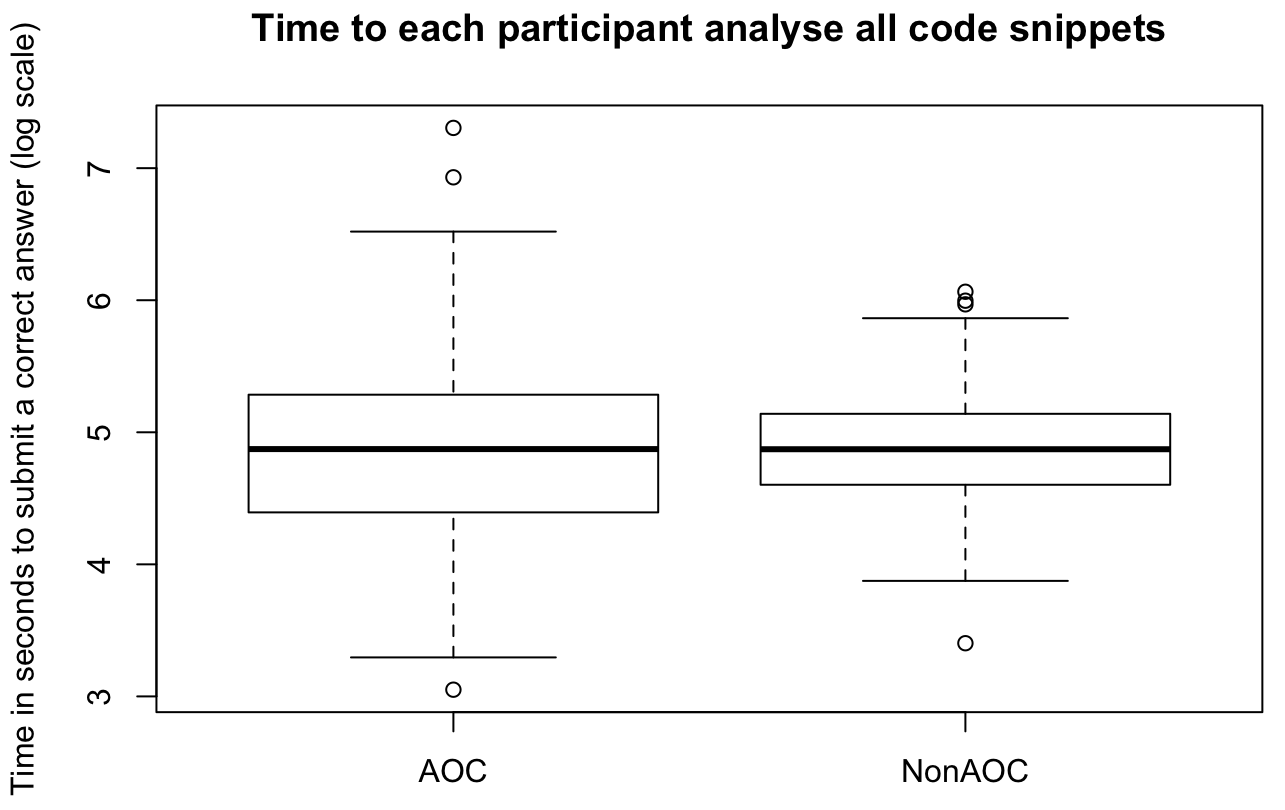
\includegraphics[scale=.20]{images/timeeach.png}
      \caption{Box plot of time to answer each snippet}
      \label{fig:timetoanswer}
  \end{figure}
    
Recalling our second research question of this survey (\emph{Do code snippets with atoms of confusion require programmers to take longer to predict their output?}), the variance in the time to correctly predict the output of a snippet is significantly smaller. Moreover, since the number of answers is the same for each inspected atom, data from table \ref{results_time} shows that the time taken to answer questions without atoms of confusion is 20\% smaller. Not all atoms, though, took less time to predict the answer. In fact, for the \emph{Arithmetic as Logic} and the \emph{Pre-Increment} atoms, there was an increase of 24\% and 44\% in the time taken to answer questions wherein the atoms had been removed. For other two atoms, there is no difference whatsoever in the time taken. We only find in half of our atoms an increase in the time taken to answer. Therefore, even though we are not able to confirm hypotheses H.2 defined in Section 1, further inquiry would be necessary to discover the reason for some atoms taking even longer.

\rb{talvez tenhamos que descrever e testar as hipoteses. a descricao pode ser feita na secao de study settings, e o resultado dos testes pode aparecer aqui.}

% \rb{acho que podemos melhorar a apresenta\c c\~{a}o dessas tabelas, talvez usando booktabs.}


\subsection{Results of the second study: Interview}
\label{sec:interview-results}

In this section we present the results of two rounds of two rounds of interviews with practitioners who agreed to participate in the interviews.In the first interview, a total of 15 practitioners were surveyed. In this phase, we collected information regarding programming experience, familiarity with JavaScript, and we also collected their opinions regarding nine candidates to atoms of confusion. This was done by presenting them pairs of code snippets whose behavior was identical, and ask them to classify each snippets readability.

In the second round of interviews, ten of the fifteen developers who participated in the first round were shown another 8 candidates to atom of confusion whose frequency we observed during the repository mining phase. The same procedure of showing code that behaves exactly the same and surveying for how easy to understand each snippet was applied in this phase. 

Supporting the results of the survey,Tables \ref{tab:interview-results1} and \ref{tab:interview-results2} show that for twelve out of the seventeen scenarios surveyed, the respondents prefer the version of the code without the atom of confusion, and in no case the \emph{neutral} ratio was higher than the option for the version without atoms of confusion.An example entry is contained in Appendix~\ref{}. 
For a full listing of the code snippets, visit the paper repository. 

\subsubsection*{Participants views of the atoms} Interesting, only for the \emph{ternary operator} scenario the participants prefer the version of the code with the atom of confusion, instead of the more cleaner version without the atom of confusion. Even in this case, some participants who opted for the \emph{left-hand-side} (with the atom of confusion) version still believed that the \emph{right-hand-side} (without the atom of confusion) version was more readable (see Figure~\ref{code:ternary}). 
The following quotes were extracted from three interviews:

\begin{figure*}

\noindent\begin{minipage}{.45\textwidth}
\begin{lstlisting}[language=JavaScript, caption=\emph{Left-hand side} (using the \emph{Ternary Operator} atom)]
let config = {size: 3, isActive: false};
const_config = config.isActive === true 
             ? config 
             : {size: 10};
console.log(_config.size);
\end{lstlisting}
\end{minipage}\hfill
\begin{minipage}{.45\textwidth}
\begin{lstlisting}[language=JavaScript, caption=\emph{Right-hand side} (without the atom)]
let config = {size: 3, isActive: false}
let _config;
if(config.isActive === true) {
  _config = config;
}
else{
   _config = {size: 10};
}
console.log(_config.size);
\end{lstlisting}
\end{minipage}
\caption{Example of pair of code snippets used in the interview. This case explores the use of the \emph{Ternary Operator atom of confusion}}
\label{code:ternary}
\end{figure*}

\begin{mq}
\emph{``I prefer to write [code using the \lhs version], but I think [the \rhs version]  is easier to read, especially for newer programmers".}
\end{mq}

\begin{mq}
\emph{``When I am programming, I write code with the ternary operator, [...], but, to be honest, I still think that the [the code using the \lhs version] is easier to understand"}.
\end{mq}

\begin{mq}
\emph{``I think [the \lhs version] is easier to understand, but [the \rhs version] is what I would write"}
\end{mq}

This particular atom of confusion also opens up the possibility for a derivative construct that JavaScript allows which can be rather confusing, and that is the nested ternaries construct, in which the right-hand side of the a ternary operator can be another ternary construct. While nested ternaries remove the number of lines that would be necessary to construct using nested if-then-else statements, they can become quite taxing, cognitively speaking, to understand. Therefore, nested ternaries are a choice of atoms to be analysed in future work.

\rb{Poder\'{i}amos quantificar a existencia de emph{nesting} com code queries?}

The \emph{Pre-Increment} atom of confusion also caused such divide in one of the interviewees, as they regarded the \emph{\rhs version} (without atom of confusion) as simpler to understand, but would still opt to write code that contained the atom. In contrast to such opinion, one of the participants found the version that contained the atom of confusion more elegant, but recognized it was less readable, and was willing to sacrifice elegance for readability.

When analyzing the \emph{Logic as Control Flow} atom of confusion, one of the interviewees gave an example of his own experience on why one should avoid writing code with such atom:

\begin{mq}
\emph{``This one is interesting, because I have written code that looks like the [\lhs version (with the atom of confusion)], and my colleagues complained that it was difficult to understand. So nowadays I prefer to write code using the [\rhs version]."}
\end{mq}

Two of the atoms had unanimous preference for the versions that did not contain the atoms: \emph{Comma Operator} and \emph{Omitted Curly Braces and Indentation}. Regarding the first one, we could often notice during the interviews that the \emph{\lhs} (with the atom of confusion) caused significant confusion among the participants. Two remarks about the \emph{Comma Operator} atom of confusion are listed below:

\begin{mq}
\emph{``I just learned that [the \lhs version of this code] is possible. I did not even know it worked"}
\end{mq}

\begin{mq}
\emph{``The code in [the \lhs version] is unlikely to be understood unless the programmer knows \clang or \cpplang"}
\end{mq}

As for the \emph{Omitted Curly Braces and Indentation} atom of confusion, which, as we shall see in Section~\ref{sec:msr-results}, is frequent in JS code bases, one of the interviewees mentioned that, although they understand why one would opt to not use braces for simple if-then-else statements, he still advised against it, on grounds that:

\begin{mq}
\emph{``[I prefer the \rhs version of the code \ldots] If I want to see well-written, easily understandable code, then I also have to do my job. Therefore I believe that, since I do not know who is on the other end maintaining this code, and it could be any person with any level of expertise, then I try to write readable, easy-to-understand code"}
\end{mq}

This view is central to our research on why such small, yet tricky, constructs should be avoided whenever possible, since maintenance is one of the longer and most costly parts of the software development life cycle, and one cannot make any assumptions about the other programmers' experience.

\rb{que conclus\~{a}o extra\'{i}mos com essa parte do estudo?} 


\subsection{Common Remarks From the Open-ended Questions} The final remarks that were drawn from the interviews are related to potentially confusing constructs that were suggested by the participants, as well as their perspective on JavaScript as a language, from which we can also uncover some other forms in which the language itself might contribute to writing confuse code.

One of the participants mentioned that the use of JavaScript's prototype-based inheritance can make it difficult to understand code that, particularly when involving  deep prototype chains. This is a core feature of the language, and most high-level tools and frameworks abstract it away. Although this was only mentioned by one practitioner, this is an important remark, as true understanding of JavaScript software necessarily involves understanding the concept of prototypes.

When asked about particular JavaScript constructs or patterns that can make code difficult to understand, three participants cited the callback pattern, which can lead to several levels of nested function calls, as extremely difficult to assimilate. One of the respondents regarded nested callbacks difficult even to write:

\begin{mq}
\emph{``Nested callbacks are very confusing. Even writing them can be confusing, let alone understanding them."}
\end{mq}

Two other developers implicitly touched upon the callback pattern, mentioning that it can be difficult to understand 'asynchronous' programming in JavaScript. Since what is really happening at a lower level is that the JavaScript engine creates a callback stack that is separate from the main execution stack, and that callback functions are only executed when the main execution stack is empty, the concepts of asynchronous events and callbacks are inseparable in the language, and any abstractions for callback functions, such as promises and async/await syntax only hide the pattern.

% citar uninitialized objects' types. floating point precision issues, 'this', type coercion

% \subsection{Common Misunderstandings About the Language}

A total of 40\% (n = 6) practitioners regarded the JavaScript language as quick and/or easy to learn, and 26.7\%(n = 4) mentioned that the abundance of frameworks, coupled with the abstractions they provide, make it so that one can develop quickly in the language. However, as mentioned by one of the interviewees, ``\emph{Developers who have started programming in JavaScript might miss out on important lower-level aspects, such as garbage collection, memory management, and processor management.}''. 

Moreover, such abstractions can make it so that one starts to program using the language without actually understanding some of its basic aspects. For instance, 26.7\%(n = 4) said that the language is not typed, 13.3\%(n = 2) believed the language runs exclusively on browsers, and two other developers stated that the language is natively asynchronous, all of which are incorrect statements. For the multi-purpose language that is one of the most, if not the most used one by practitioners
~\cite{}, a lack of understanding of the languages core features may be a problem worth investigating in future studies.

\rb{seria importante apresentar uma conclus\~{a}o em rela\c c\~{a}o a essa parte do estudo. Acredito que seja interessante discutir um pouco essa ``faca de dois gumes'' sobre a flexibilidade, mencionada abaixo. }

\adriano{Fiquei em duvida se vale citar os contras mais interessantes que os entrevistados falaram sobre JS: (1x) o jeito como ela lida com 'this', (que esta ligado a ela ser puramente orientada a objetos, sem classe); (2x)falta de precisao para tratamento de ponto flutuante, o que pode a tornar inadequada para tratamento de dados/ciencias puras; e a faca de dois gumes que e a flexibilidade da linguagem: muitos falavam isso como ponto positivo e negativo ao mesmo tempo. \todo[inline]{eu acho que podemos mencionar sim}}

\begin{table}[!htb]
    \centering
    \caption{Interviews Round 1 - Summary of participants' preferences for code snippets \textsc{with} and \textsc{without} atoms of confusion (\textsc{aoc}). Participants were also allowed to choose \textsc{neutral} when they thought both sides were equally readable.}
    \label{tab:interview-results1}
    \begin{tabular}{lrrr}\toprule
      & \multicolumn{3}{c}{\textsc{Preference (\%)}} \\
      \cmidrule(lr){2-4}
         \textsc{atom}           & \multicolumn{1}{c}{\textsc{with aoc}}
                                      &  \multicolumn{1}{c}{\textsc{without aoc}}
                                               & \multicolumn{1}{c}{\textsc{neutral}} \\ \midrule
         Arithmetic as Logic     & 0  & 93.33  & 6.67  \\
         Assignment as Value     & 20 & 60     & 20    \\
         Comma Operator          & 0  & 100    & 0     \\
         Ternary Operator        & 60 & 26.67  & 13.3  \\
         Implicit Predicate      & 20 & 73.33  & 6.67  \\
         Logic as Control Flow   & 20 & 60     & 20    \\
         Omitted Curly Braces    & 0  & 100    & 0     \\
         Post Increment          & 20 & 73.33  & 6.67  \\
         Pre Increment           & 40 & 46.67  & 13.33 \\ \midrule
         \textsc{overall}        & 20 & 70.37  & 9.63  \\
         \bottomrule
    \end{tabular}
\end{table}

\begin{table}[!htb]
    \centering
    \caption{Interviews Round 2 - Summary of participants' preferences for code snippets \textsc{with} and \textsc{without} atoms of confusion (\textsc{aoc}). Participants were also allowed to choose \textsc{neutral} when they thought both sides were equally readable.}
    \label{tab:interview-results2}
    \begin{tabular}{lrrr}\toprule
      & \multicolumn{3}{c}{\textsc{Preference (\%)}} \\
      \cmidrule(lr){2-4}
         \textsc{atom}           & \multicolumn{1}{c}{\textsc{with aoc}}
                                      &  \multicolumn{1}{c}{\textsc{without aoc}}
                                               & \multicolumn{1}{c}{\textsc{neutral}} \\ \midrule
         Property access         & 10  & 60  & 30  \\
         Object spread           & 50 & 50     & 0    \\
         Array spread            & 60  & 40    & 0     \\
         Arrow function          & 40 & 40     & 20  \\
         Array destructuring     & 40 & 40  & 20  \\
         Object destructuring    & 40 & 40     & 20    \\
         Type conversion         & 30  & 60    & 10     \\
         Change Literal encoding & 40 & 50  & 10  \\ \midrule
         \textsc{overall}        & 42.8 & 47.6  & 9.6  \\
         \bottomrule
    \end{tabular}
\end{table}

\subsection{Results of the third study: Mining open source repositories}
\label{sec:msr-results} 

We mined \minedprojects open source JavaScript repositories to understand how often atoms of confusion arise in real software. Similarly to a previous study~\cite{DBLP:conf/msr/GopsteinZFC18}, which investigates the prevalence of atoms of confusion in open source \clang and \cpplang projects, we found that atoms of confusion frequently arise in JavaScript open source systems. 

The 3 most frequently found atoms occur in at least 80\% of the projects.
Considering the extremes, atom Ternary Operator was found in 89.69\% of the repositories, while atom Comma Operator occurred in only 11.34\% of them (as seen in Figure~\ref{fig:rate}).

% Figure~\ref{fig:rate} summarizes this finding, showing that the occurrence of atoms of confusion in JavaScript systems range from 11.34\% (Comma Operator) to 89.69\% (Ternary Operator).


%Figure~\ref{fig:atoms-occurrence} shows that the occurrence of in JavaScript systems range from 

\begin{figure}
    \centering
    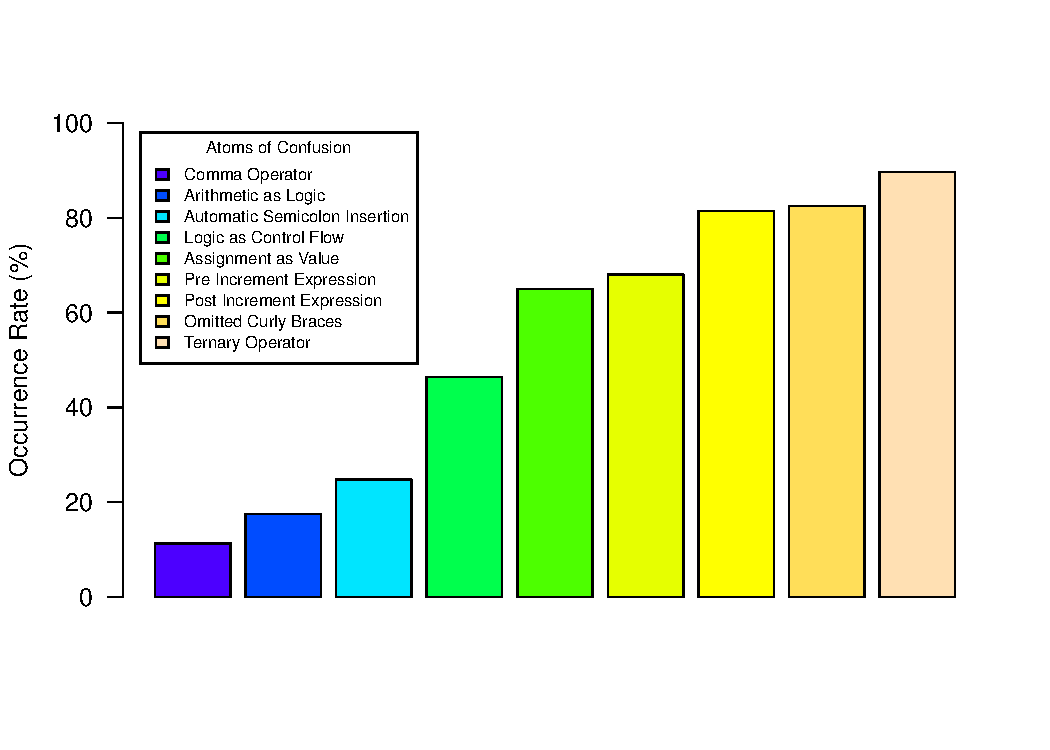
\includegraphics[width=\columnwidth]{images/rate-1.pdf}
    \caption{Incidence of atoms of confusion across the \minedprojects JavaScript repositories we mined}
    \label{fig:rate}
\end{figure}

\begin{figure}
    \centering
    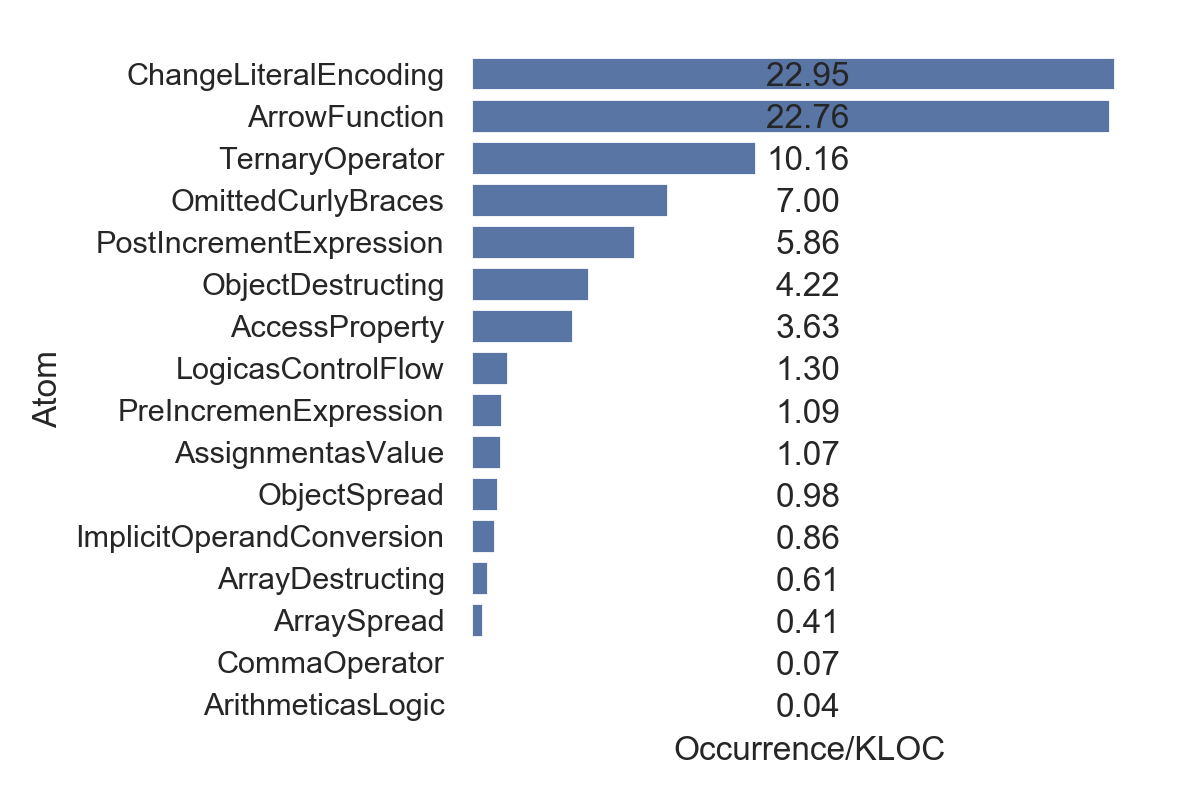
\includegraphics[width=\columnwidth]{images/chart_ocurrence_kloc.png}
    \caption{The rate of each atom per thousand lines of code (KLOC) across all \minedprojects repositories}
    \label{fig:atoms-occurrence}
\end{figure}


Considering all JavaScript projects in our dataset, we found 
a total of \num{206317} atoms of confusion, though three atoms are responsible for 87.47\% of this total: Post Increment Expression, Omitted Curly Braces, and the Ternary Operator. The remaining atoms accounts for \num{25851} (12.53\%) of the total number of occurrences, and the Comma Operator and and Arithmetic as Control Flow are the atoms that arise less frequently (0.25\% in total with 373 and 164 occurrences, respectively).
%In our dataset of JavaScript projects, 
We found the Ternary Operator atom occurring more frequently than the Omitted Curly Braces, differently from what has been reported in a previous work~\cite{DBLP:conf/msr/GopsteinZFC18}. 

The results of our survey and interviews suggest that the Ternary Operator does not contribute significantly as a source of misunderstanding (increasing the number of wrong answers in 9\% of the cases, according to our survey). Nonetheless, the Post Increment Expression and Omitted Curly Braces atoms are listed in the top three sources of misunderstanding 
(see Table~\ref{tab:difference-correctness}). As such, fixing the the Post Increment Expression and Omitted Curly Braces might solve most of the unclear code caused by atoms of confusion. 

\rb{continuar desse ponto}


\subsection{Discussion}
\label{sec:discussion}
